\documentclass[11pt,twoside,a4paper]{book}  
% definice dokumentu
\usepackage[czech, english]{babel}
\usepackage[T1]{fontenc} 				% pouzije EC fonty 
\usepackage[utf8]{inputenc} 			% utf8 kódování vstupu 
\usepackage[square, numbers]{natbib}	% sazba pouzite literatury
\usepackage{indentfirst} 				% 1. odstavec jako v cestine, pro práci v aj možno zakomentovat
\usepackage{fancyhdr}					% tisk hlaviček a patiček stránek
\usepackage{nomencl} 					% umožňuje snadno definovat zkratky a jejich seznam


%%%%%%%%%%%%%%%%%%%%%%%%%%%%%%%%%%%%%%%%%%%%%%%%%%%%%%%%%%%%%%%
% informace o práci
\newcommand\WorkTitle{Servisně orientovaný aspektový vývoj uživatelských rozhraní pro mobilní aplikace}		% název
\newcommand\FirstandFamilyName{Pavel Matyáš}															% autor
\newcommand\Supervisor{Ing. Martin Tomášek}															% vedoucí

\newcommand\TypeOfWork{Bakalářská práce}	% typ práce [Diplomová práce | Bakalářská práce | Bachelor's Project | Master's Thesis ]	

% Nastavte následují podle vašeho oboru a programu (pomoc hledejte na http://www.fel.cvut.cz/cz/education/bk/prehled.html)								
\newcommand\StudProgram{Otevřená informatika, Bakalářský}	% program
\newcommand\StudBranch{Softwarové inženýrství}           					% obor

%%%%%%%%%%%%%%%%%%%%%%%%%%%%%%%%%%%%%%%%%%%%%%%%%%%%%%%%%%%%%%%
% minimální importy
\usepackage{graphicx}					% pro vkládání obrázků
\usepackage{k336_thesis_macros} 		% specialni makra pro formatovani DP a BP
\usepackage[
pdftitle={\WorkTitle},				% nastaví v informacích o pdf název
pdfauthor={\FirstandFamilyName},	% nastaví v informacích o pdf autora
colorlinks=true,					% před tiskem doporučujeme nastavit na false, aby odkazy a url nebyly šedé při ČB tisku
breaklinks=true,
urlcolor=red,
citecolor=blue,
linkcolor=blue,
unicode=true,
]
{hyperref}								% pro zobrazování "prokliknutelných" linků 

% rozšiřující importy
\usepackage{listings} 			%slouží pro tisk zdrojových kódů se syntax higlighting
\usepackage{algorithmicx} 		%slouží pro zápis algoritmů
\usepackage{algpseudocode} 		%slouží pro výpis pseudokódu

%%%%%%%%%%%%%%%%%%%%%%%%%%%%%%%%%%%%%%%%%%%%%%%%%%%%%%%%%%%%%%%
% příkazy šablony
\makenomenclature								% při překladu zajistí vytvoření pracovního souboru se seznamem zkratek

\let\oldUrl\url									% url adresy budou zobrazeny: <url> 
\renewcommand\url[1]{<\texttt{\oldUrl{#1}}>}

%%%%%%%%%%%%%%%%%%%%%%%%%%%%%%%%%%%%%%%%%%%%%%%%%%%%%%%%%%%%%%%
% vaše vlastní příkazy
\newcommand*{\nomExpl}[2]{#2 (#1)\nomenclature{#1}{#2}} 	% usnadňuje zápis zkratek : Slova ke Zkrácení (SZ)
\newcommand*{\nom}[2]{#1\nomenclature{#1}{#2}} 			% usnadňuje zápis zkratek : SZ



%%%%%%%%%%%%%%%%%%%%%%%%%%%%%%%%%%%%%%%%%%%%%%%%%%%%%%%%%%%%%%%
% vlastní dokument
%%%%%%%%%%%%%%%%%%%%%%%%%%%%%%%%%%%%%%%%%%%%%%%%%%%%%%%%%%%%%%%
\begin{document}
	
	%%%%%%%%%%%%%%%%%%%%%%%%%% 
	% nastavení jazyka, kterým je práce psána
	\selectlanguage{czech}	% podle jazyka práce nastavte na [czech | english]
	\translate				% nastaví české nebo anglické popisy (např. katedra -> department); viz k336_thesis_macros

	%%%%%%%%%%%%%%%%%%%%%%%%%%    
	% Poznamky ke kompletaci prace
	% Nasledujici pasaz uzavrenou v {} ve sve praci samozrejme 
	% zakomentujte nebo odstrante. 
	% Ve vysledne svazane praci bude nahrazena skutecnym 
	% oficialnim zadanim vasi prace.
	{
	\pagenumbering{roman} \cleardoublepage \thispagestyle{empty}
	\chapter*{Na tomto místě bude oficiální zadání vaší práce}
	\begin{itemize}
		\item Toto zadání je podepsané děkanem a vedoucím katedry,
		\item musíte si ho vyzvednout na studijním oddělení Katedry počítačů na Karlově náměstí,
		\item v jedné odevzdané práci bude originál tohoto zadání (originál zůstává po obhajobě na katedře),
		\item ve druhé bude na stejném místě neověřená kopie tohoto dokumentu (tato se vám vrátí po obhajobě).
	\end{itemize}
	\newpage
	}

	%%%%%%%%%%%%%%%%%%%%%%%%%%    
	% Titulni stranka / Title page 
	\coverpagestarts

	%%%%%%%%%%%%%%%%%%%%%%%%%%%    
	% Poděkovani / Acknowledgements 

	\acknowledgements
	\noindent
	Zde můžete napsat své poděkování, pokud chcete a máte komu děkovat.


	%%%%%%%%%%%%%%%%%%%%%%%%%%%   
	% Prohlášení / Declaration 

	\declaration{V~Kořenovicích nad Bečvárkou dne 15.\,5.\,2008}
	%\declaration{In Kořenovice nad Bečvárkou on May 15, 2008}


	%%%%%%%%%%%%%%%%%%%%%%%%%%%%    
	% Abstrakt / Abstract 
 
	\abstractpage

	Translation of Czech abstract into English.

	% Prace v cestine musi krome abstraktu v anglictine obsahovat i
	% abstrakt v cestine.
	\vglue60mm

	\noindent{\Huge \textbf{Abstrakt}}
	\vskip 2.75\baselineskip

	\noindent
	Abstrakt práce by měl velmi stručně vystihovat její obsah. Tedy čím se práce zabývá a co je jejím výsledkem/přínosem.

	\noindent
	Očekávají se cca 1 -- 2 odstavce, maximálně půl stránky.

	%%%%%%%%%%%%%%%%%%%%%%%%%%    
	% obsahy a seznamy
	\tableofcontents		% Obsah / Table of Contents 

	% pokud v práci nejsou obrázky nebo tabulky - odstraňte jejich seznam
	\listoffigures			% Obsah / Table of Contents 
	\listoftables			% Seznam tabulek / List of Tables

	%%%%%%%%%%%%%%%%%%%%%%%%%% 
	% začátek textu  
	\mainbodystarts
%**************************************************************

% Pro snadnejsi praci s vetsimi texty je rozumne tyto rozdelit
% do samostatnych souboru nejlepe dle kapitol a tyto potom vkladat
% pomoci prikazu \include{jmeno_souboru.tex} nebo \include{jmeno_souboru}.
% Napr.:
% \chapter{Úvod}
Tato bakalářská práce se zabývá analýzou, návrhem a otestováním frameworků pro mobilní platformy Android a Windows Phone. Tyto frameworky interpretují uživatelské rozhraní z dat generovaných serverem z modelu, která jsou poskytována serverem pomocí webových služeb.

První část práce popisuje aktuální situaci v tvorbě UI, specifikuje požadavky a cíle práce a zkoumá již existující řešení. V druhé části se analyzují požadavky, které by měla práce splňovat, a návrh řešení, které stanovené požadavky a cíle splňuje. Ve třetí části je popsána struktura a vlastní implementace řešení. Poslední část obsahuje otestování řešení a ukazuje vzorové aplikace na dvou různých mobilních prostředích.

Práce obsahuje seznam použitých zkratek, které lze nalézt v příloze A, instalační příručku v příloze B, použité UML diagramy a obrázky viz příloha C, ukázky zdrojových kódů v příloze D a obsah CD s prací a zdrojovými kódy je v příloze E.
 
\section{Motivace}
Nedílnou součástí většiny dnešních aplikací je uživatelské rozhraní. Uživatelské rozhraní by mělo uživateli co nejvíce usnadňovat manipulaci se softwarem a tudíž být intuitivní a použitelné, mělo by mít adekvátní design, nejlépe korespondující s aktuálními trendy. Vývoj takového rozhraní je však časově velmi náročný proces, který zahrnuje nejenom samotný vývoj, ale také rozsáhlé testování, hlavně z hlediska funkčnosti a použitelnosti. Celý problém navíc umocňuje fakt, že se vývojáři snaží zajistit podporu softwaru na více platformách, neboť chtějí uživatelům nabídnout možnost operovat s jejich vytvořeným systémem nejen z počítače či laptopu, ale také z tabletu nebo mobilního zařízení. Mobilní verze grafického uživatelského rozhraní nebývá často moc rozdílná od rozhraní ostatních platforem v tom smyslu, že se v ní vyskytují převážně stejné grafické prvky, a tak pro mobilní verzi vzniká téměř indentická kopie tohoto rozhraní, což vede i k duplicitě v kódu aplikace \cite{on-web-services}. Problémem je, že se často uživatelská rozhraní mění, ať už se změna týká rozložení komponent, přidání nebo odebrání komponenty nebo třeba validace uživatelského vstupu, protože takováto změna se musí provést na všech platformách a někdy i na více místech v rámci aplikace, což může být v případě rozsáhlých systémů nejednoduchý úkol, který stojí vývojáře spoustu zbytečného času a může vést i ke vzniku nových typů chyb \cite{towards-smart-design}. Pokud bychom byli schopni nadefinovat uživatelské rozhraní jen jednou pro všechny platformy na jednom místě, tento problém bychom odstranili. Definice by tedy byla obecná, ale každá platforma je jiná a něčím specifická, proto je třeba vytvořit pro různé platformy frameworky, které obecnou definici pro danou platformu interpretují. 

Bylo mi nabítnuto vytvořit takovýto framework pro dvě mobilní platformy, kontrétně pro Android a Windows Phone, což mi přislo velmi užitečné a zajímavé, a proto jsem se rozhodl zpracovat toto téma jako bakalářskou práci.

% \include{2_teorie}
% atd...

%*****************************************************************************
\chapter{Úvod}
Tato bakalářská práce se zabývá analýzou, návrhem a otestováním frameworků pro mobilní platformy Android a Windows Phone. Tyto frameworky interpretují uživatelské rozhraní z dat generovaných serverem z modelu, která jsou poskytována serverem pomocí webových služeb.

První část práce popisuje aktuální situaci v tvorbě UI, specifikuje požadavky a cíle práce a zkoumá již existující řešení. V druhé části se analyzují požadavky, které by měla práce splňovat, a návrh řešení, které stanovené požadavky a cíle splňuje. Ve třetí části je popsána struktura a vlastní implementace řešení. Poslední část obsahuje otestování řešení a ukazuje vzorové aplikace na dvou různých mobilních prostředích.

Práce obsahuje seznam použitých zkratek, které lze nalézt v příloze A, instalační příručku v příloze B, použité UML diagramy a obrázky viz příloha C, ukázky zdrojových kódů v příloze D a obsah CD s prací a zdrojovými kódy je v příloze E.
 
\section{Motivace}
Nedílnou součástí většiny dnešních aplikací je uživatelské rozhraní. Uživatelské rozhraní by mělo uživateli co nejvíce usnadňovat manipulaci se softwarem a tudíž být intuitivní a použitelné, mělo by mít adekvátní design, nejlépe korespondující s aktuálními trendy. Vývoj takového rozhraní je však časově velmi náročný proces, který zahrnuje nejenom samotný vývoj, ale také rozsáhlé testování, hlavně z hlediska funkčnosti a použitelnosti. Celý problém navíc umocňuje fakt, že se vývojáři snaží zajistit podporu softwaru na více platformách, neboť chtějí uživatelům nabídnout možnost operovat s jejich vytvořeným systémem nejen z počítače či laptopu, ale také z tabletu nebo mobilního zařízení. Mobilní verze grafického uživatelského rozhraní nebývá často moc rozdílná od rozhraní ostatních platforem v tom smyslu, že se v ní vyskytují převážně stejné grafické prvky, a tak pro mobilní verzi vzniká téměř indentická kopie tohoto rozhraní, což vede i k duplicitě v kódu aplikace \cite{on-web-services}. Problémem je, že se často uživatelská rozhraní mění, ať už se změna týká rozložení komponent, přidání nebo odebrání komponenty nebo třeba validace uživatelského vstupu, protože takováto změna se musí provést na všech platformách a někdy i na více místech v rámci aplikace, což může být v případě rozsáhlých systémů nejednoduchý úkol, který stojí vývojáře spoustu zbytečného času a může vést i ke vzniku nových typů chyb \cite{towards-smart-design}. Pokud bychom byli schopni nadefinovat uživatelské rozhraní jen jednou pro všechny platformy na jednom místě, tento problém bychom odstranili. Definice by tedy byla obecná, ale každá platforma je jiná a něčím specifická, proto je třeba vytvořit pro různé platformy frameworky, které obecnou definici pro danou platformu interpretují. 

Bylo mi nabítnuto vytvořit takovýto framework pro dvě mobilní platformy, kontrétně pro Android a Windows Phone, což mi přislo velmi užitečné a zajímavé, a proto jsem se rozhodl zpracovat toto téma jako bakalářskou práci.

\chapter{Popis problému a specifikace cíle}
\section{Popis problematiky}

Softwarový systém má sloužit člověku k řešení nějakého problému. Uživatel přitom často problém blíže specifikuje a systém musí mít způsob, jak uživateli sdělit jeho řešení. K tomu slouží uživatelská rozhraní, která umožňují vzájemnou komunikaci systému s uživatelem. Uživatelské rozhraní přitom není jednoduchá záležitost. V první řadě by mělo být navrženo tak, aby sloužilo uživateli. Mělo by mu umožnit jednoduchou interakci se systémem, být intuitivní, funkční a hlavně použitelné. 


\subsection{Různá uživatelská rozhraní}
Aby bylo uživatelské rozhraní použitelné a uživatelsky přívětivé je třeba prozkoumat, jakým způsobem člověk s aplikacemi spolupracuje. Nejen tímto se zabývá disciplína zvaná Human Computer Interaction, která zkoumá potřeby uživatelů z různorodých hledisek. Díky této disciplíně vzniklo množství uživatelských rozhraní, pomocí kterých může člověk s počítačem komunikovat. Jedním z takových rozhraní je textové uživatelské rozhraní, značené CUI, jehož typickým zástupcem je příkazová řádka. Dalším typem je Hlasové uživatelské rozhraní, které dokáže interpretovat povely zadané lidskou řečí. Nejrozšířenějším je však grafické uživatelské rozhraní, zkráceně GUI, které využívá grafické prvky. GUI se stalo velmi oblíbeným právě proto, že je jednoduché a grafické prvky v člověku vyvolávají podobnost s vnějším světem. Také není nutné znát žádně specifické příkazy, jako v případě příkazové řádky, nebo hlasové povely jako v případě hlasového rozhraní. Zmínil bych ještě multimodální rozhraní, která používají k interakci více lidských smyslů a tak jsou vhodná například i pro lidi s postižením \cite{uiTypes}. 

V softwarových systémech je nejběžnějsím způsobem interakce uživatele se systémem právě grafické uživatelské rozhraní a tím se taky v této práci zabýváme. Návrh GUI je potřeba důkladně zvážit, neboť závisí na mnoha aspektech. Důležité je, pro jaké zařízení GUI tvoříme, jaký účel má aplikace, která bude rozhraním disponovat a také stav uživatele a prostředí, ve kterém se nachází. Typ zařízení je důležitý hlavně proto, protože každé zařízení používá jiné ovládací prvky. Zatímco u mobilního zařízení můžeme očekávat použití dotykového displeje, u počítače zase použití myši, klávesnice nebo dokonce jiných externích vstupních zařízení, jako může být například grafický tablet. Také je třeba vzít v potaz jinou velikost displeje a jiná rozlišení jednotlivých zařízení. Účel aplikace ovlivňuje GUI hlavně z hlediska obsahu, tedy jaké komponenty je nutné mít, aby byla aplikace využívána k daném účelu. Těžko by asi někdo chtěl emailového klienta bez možnosti odeslat zprávu. Stav uživatele a prostředí může zase ovlivnit způsob ovládání aplikace. Příkladem může být palubní počítač v automobilu, na kterém by měl uživatel být schopen přepnout rádiovou stanici, aniž by se přestal věnovat řízení. 

Co ale takové grafické rozhraní nejčastěji obsahuje? Běžně GUI disponuje ovládacími a vizuálními prvky pomocí kterých lze aplikaci ovládat. Osobně bych GUI prvky rozdělil na vstupní a výstupní. Vstupní prvky zachycují uživatelský vstup a akce, které systém ovládají a výstupní zobrazují uživateli výsledky těchto akcí, data a aktuální stav systému. Vstupními prvky jsou nejčastěji vstupní pole, do kterých může uživatel napsat text, něco zaškrtnout, vybrat mezi možnostmi atp. Takovéto skupině vstupních polí se říká formulář. Systém samozřejmě může pole ve formuláři předvyplnit a z polí tak udělat výstupní prvky, které rovněž budou uživatele informovat o stavu systému. Dalšími vstupními prvky jsou také tlačítka, které provádějí dané akce jako například odeslání formuláře. Výstupními prvky jsou například statické texty, tabulky nebo seznamy položek. 

Pro pořádek, v textu budu používat zkratky GUI i UI, kterými budu bez rozdílu myslet grafické uživatelské rozhraní nikoli tedy jinou formu zmíněnou v této sekci.

\subsection{Tvorba uživatelského rozhraní}

Tvorba uživatelského rozhraní není vůbec jednoduchá záležitost. Vývojáři vkládají do tvorby uživatelského rozhraní velké úsilí a značné množství času. Bylo zjištěno, že uživatelské rozhraní zabírá přibližně 48\% kódu aplikace a zhruba 50\% času, který vývoji aplikace věnujeme \cite{towards-smart-design}. Další čas a úsilí také zabere testování rozhraní hlavně z hlediska použitelnosti, které opět stojí spoustu času a nákladů. Například vývojář mnohdy nedokáže odhadnout chování cílové skupiny, která systém bude používat, a tak se často dělají testy s koncovým uživatelem, u kterých se zkoumá, jak daný uživatel software ovládá. Z těchto testů často odhalíme, že uživatelské rozhraní je nedostačující a neposkytuje uživateli komfort při ovládání systému, který by poskystkout mělo. Z vlastní zkušenosti s tímto testem také vím, že velkým problémem je uživatelský vstup, který musí být validován, aby uživatel nevložil data, která jsou v rozporu s modelem, na který je rozhraní namapováno \cite{cernyTEA}. Také je žádoucí zobrazovat uživateli pouze to, co by vidět měl, například na základě jeho uživatelské role v systému. V neposlední řadě je také důležité, jak rozhraní vypadá. Důležitým aspektem rozhraní je, jakým způsobem jsou v něm reprezentována data , a také jak jsou uspořádány jeho jednotlivé části. Z výše uvedeného lze vidět, že je tvorba uživatelského rozhraní opravdu náročný a rozsáhlý proces. Právě proto je poskytovat pro systém více verzí uživatelských rozhraní, například pro různé platformy nebo pro různé uživatelské role, obtížný úkol \cite{cernyTEA}.

Softwarový systém se po nasazení musí také dále udržovat. Ne nadarmo je jedním z hlavních a kritických aspektů dobrého softwaru jeho udržovatelnost, anglicky Maintainability. Udržovatelnost můžeme definovat jako schopnost systému se dále měnit a vyjívet na základě požadavků zákazníka. Změny by přitom měly být lehce proveditelné a něměly by nějak výrazně ovlivnit stav systému. Požadavky na změnu lze očekávat vždy, neboť nevyhnutelně vznikají jako reakce na změny v podnikatelském prostředí (http://faculty.mu.edu.sa/public/uploads/1429431793.203Software%20Engineering%20by%20Somerville.pdf strana 8). Neboli musíme provést změny, jinak nás konkurence předčí. Bohužel však uživatelské rozhraní tuto vlastnost moc nesplňuje. 
Mějme například desktopovou a mobilní aplikaci, které obě obsahují formulář namapovaný na určitou entitu v databázovém modelu. Tento model se nějak změní, například v dané entitě rozdělíme jeden sloupec na dva. Naneštěstí neexistuje žádný machanismus, který by automaticky zaručil, že je UI v souladu s modelem \cite{cernyTEA}. Z pohledu vývojáře to pak znamená, že pokud změní databázový model, musí také změnit uživatelské rozhraní v obou klientských aplikacích, aby korespondovalo s novým databázovým modelem, což je jistá forma typové kontroly. Zde nejenom, že musí vývojář udělat dvakrát stejnou věc, ale také může udělat chybu, což vyústí v nefunkčnost systému. Také pokud se takový formulář vyskytuje třeba na pěti místech v aplikaci, změna je už časově náročnější, hůře proveditelná a ještě více náchylná na chybu vývojáře, který může na nějaký výskyt formuláře zapomenout.
Takovým zásahem do systému nemusí být jen změna databázového modelu, ale také změna validací uživatelského vstupu, které se týkají i bussiness modelu, nebo třeba změna rozložení či pořadí jednotlivých polí ve formuláři.

\subsection{Využití webových služeb pro zisk a odeslání dat}
Jak už bylo řečeno v grafickém uživatelském rozhraní máme výstupní grafické prvky, jako například tabulky či seznamy položek. Tyto komponenty jsou určeny k tomu, aby zobrazovaly uživateli určitá data. Otázkou je odkud se tato data berou. Je hned několik způsobů, kde mohou být data uložena. Jednou z možností je, že má aplikace vlastní databázi. Takováto aplikace není určena k tomu, aby komunikovala nebo sdílela data s dalšími instancemi této aplikace na jiných zařízeních. Pokud komunikaci chceme, je vhodná architektura klient-server. Server může mít vlastní databázi, ze které poskytuje klientům informace například prostřednictvím webových služeb. Webová služba umožňuje jednomu zařízení interakci s jiným zařízením prostřednictvím sítě\cite{wiki-ws}. V tomto případě je jedním zařízením server ,druhým klienstká aplikace a interakcí je myšlen vzájemný přenos dat. V mobilních aplikacích jsou velmi populární interpretací webových služeb RESTful Web Services využívající Representional State Transfer (REST), který byl navržen tak, aby získával data ze zdrojů pomocí jednotných identifikátorů zdrojů (URI), což jsou typicky odkazy na webu. Využívá se právě v aplikacích s klient-server architekturou a ke komunikaci používá HTTP protokol. Výhodou využití HTTP protokolu je, že jeho metody poskytují jednotné rozhraní pro manipulaci se zdroji dat. Http metoda PUT se využívá k vytvoření nového zdroje, DELETE zdroj maže, GET se používá pro získání aktuálního stavu zdroje v nějaké dané reprezentaci a POST stav zdroje upravuje \cite{oracle-ws}. 

Víme tedy, že klient je schopen získat ze serveru data pomocí HTTP dotazu. Aby přijatá data mohl reprezentovat v UI, musí znát jejich strukturu., což by mohl být problém. Naštěstí jsou data ve spojitosti s RESTful službami nejčastěji přenášena ve formě XML nebo alternativně ve formě JSON\cite{ws-formats}. Zmíněné formy dat vzikají serialializací objektů, jejichž definici můžeme většinou získat z dokumentace poskytovatele webové služby, stejně tak jako formát, který pro bude pro serializaci použitý. Je také nutné znát metodu, kterou lze pro využití zdroje použít, popřípadě dodatečné parametry, kterými lze webovou službu nastavit. Tato data na klientovi můžeme zpracovat více způsoby. Jednou z možností je napsat si vlastní parser. Dalším způsobem je využít nějaké knihovny, která umí data sama deserializovat do objektu. Obdobně to funguje i v případě odesílání dat. Zdroj webové služby definuje v jakém formátu data přijme a v dokumentaci opět nalezneme definici objektu, do kterého se bude snažit data deserializovat. Z toho plyne, že klientská aplikace se i při zisku i při odesílání dat musí adaptovat na určitou, předem danou strukturu. Tedy pokud se změní struktura objektu, ze kterého serializací data vznikají a deserializuje se do něj vstup z klienta, je nutné upravit i příslušná místa v klienstké aplikaci, která zpracování a odesílání uživatelského vstupu mají nastarosti.  

Představme si nyní následující problém. Mějme server a na něm model naříklad Tým, který obsahuje dva sloupce - název týmu a počet členů. Vytvoříme si klienstkou aplikaci, která tato data získá a zobrazí, například v tabulce. Nyní se rozhodneme, že by měl přibýt sloupec, obsahující zkratku týmu. Nejdříve se na to podíváme z pohledu zisku dat. Upravíme tedy model na serveru a v datech, která jsou poskytována webovou službou, tedy přibude další hodnota. Proto musíme upravit klientskou aplikaci, aby s těmito dodatečnými daty počítala a rovněž je zobrazila v tabulce. Pokud se však rozhodneme, že se nějaký sloupec odstraní, je situace o trochu složitější. Po získání dat nám na klientovi hodnota bude chybět. Pokud nad hodnotou provádíme nějaké operace a nemáme klienta správně ošetřeného, může to vyústit i v pád aplikace.

Nyní budeme data posílat. Předpokládejme, že jsme ještě neprovedli změny výše a klient je tedy v souladu s modelem na serveru. Je důležité poznamenat, že server může určovat, které hodnoty vyžaduje. Pokud tedy přidáme novou hodnotu, kterou server označí jako povinnou, bude pokus neupraveného klienta zaslat data neúspěšný, neboť je server odmítne. Musíme tedy klienta upravit tak, aby bylo možné novou hodnotu zadat, to znamená přidat nové vstupní pole a upravit parser, či objekt, ze kterého se data připravují serializací na odeslání. Nastane-li odstranění nějakého sloupce z modelu na serveru, bude to pro klienta opět problém, protože bude zasílat data obsahující hodnotu, kterou server nezná a ten data opět odmítne. Znovu je nutné klienta upravit. 

Poznamenejme ještě, že pokaždé, kdy je nutné upravit klienta, se musí vydat nová verze aplikace. Bohužel v dnešní době je možnost aktualizaci neprovést, a to hlavně na mobilních zařízeních, příkladem může být Google Play na Androidu \cite{android-auto-update}. Když si novou verzi člověk nenainstaluje, hrozí tvůrcům buď uživatel s nefunkční aplikací nebo chyba na serveru, záleží na provedené změně. Spousta vývojářů tohle řeší třeba podmínkami na verzi aplikace. Znamená to, že na serveru je stále stará verze modelu, která podporuje starou strukturu dat? Nebo označili na serveru nová pole za nepovinná? Druhým používaným řešením je vynutit aktualizaci aplikace, což se mi zdá jako docela dobré řešení, ale i zde se vyskytují otázky. Co když člověk třeba nemá dostatek mobilních dat na stažení nové verze aplikace? Co když na aktualizaci právě nemá čas? Tento problém bychom eliminovali, pokud by server klienta informoval o tom, co vyžaduje a klient by se dynamicky těmto potřebám přizpůsobil.

\subsection{Existující řešení}
Snažil jsem se najít existující řešení pro mobilní aplikace, které by vytvářelo definici komponenty, například formuláře, na základě modelu a které by pro zisk těchto definic využívalo webových služeb. Bohužel jsem nenašel žádné řešení, které by přesně odpovídalo těmto specifikacím, uvádím však řešení, která řeší alespoň jejich část. Dále pak uvádím projekt AFSwinx \cite{citation-needed}, který sice požadavky splňuje, ale není určen pro mobilní aplikace, nýbrž pro Java SE platformu a AspectFaces \cite{aspect-faces} , z něhož AFSwinx vychází a který je v základu určen pro Java EE aplikace.

\subsubsection{Řešení z IBM developerWorks}
Článek Build dynamic user interfaces with Android and XML \cite{dynamic-android-xml} popisuje možnost dynamického vytvoření formuláře z XML souboru pro Android aplikace. Podle návodu aplikace stáhne z URL adresy určitý XML soubor, ve kterém je nadefinována struktura formuláře. Návod dále ukazuje, jak stažené XML parsovat a dynamicky vytvořit na jeho základě v aplikaci formulář. Tento způsob tedy formulář centralizuje. Pokud se tedy formulář vyskytuje na více místech v aplikaci a je třeba ho změnit, stačí upravit daný XML soubor. Bohužel není XML dokument generován automaticky z modelu a není využito k jeho získání webových služeb, jinak by tento způsob byl pro naše účely řešením. Také je škoda, že na základě návodu nebyla vytvořena žádná knihovna, kterou by Android aplikace mohly používat.

\subsubsection{PHP Database Form}
PHP Database Form \cite{phpdbform} je rozšíření pro PHP. Toto rozšíření dokáže automaticky z modelu v databázi vytvořit HTML kód formuláře, včetně validací jednotlivých polí. Umožňuje vybrat pro vytvoření pouze některou část tabulky a to pomocí SQL dotazu. Dále pak umožňuje dodatečná nastavení. Lze nastavit názvy polí, jejich viditelnost, dodat validace tam, kde nejsou, nastavit, jak se bude pole zobrazovat atd. Hlavními výhodami tohoto rozšíření jsou: menší množství kódu, jednoduché validování dat a možnost upravit si formulář dle libosti pomocí CSS. Využití vyžaduje PHP verzi 5.3 a Apache, Tomcat nebo Microsoft IIS web server. PHP Database Form podporuje všechny majoritně využívané databáze a webové prohlížeče. Dnes už by se i toto rozšíření dalo použít pro mobilní aplikace, neboť existují možnosti vytvářet multiplatformní mobilní aplikace pomocí HTML, CSS a JavaScriptu, které spouští aplikaci na mobilním zařízení v režimu webového prohlížeče. Takovou možností je například Apache Cordova \cite{apache-cordova}.

\subsubsection{AspectFaces}
AspectFaces je framework, který se snaží o to, aby bylo UI generováno na základě modelu \cite{aspectdriven}, k čemuž využívá inspekci tříd. To umožní nadefinovat UI pouze jednou a veškeré změny v modelu jsou automaticky do uživatelského rozhraní reflektovány. UI lze nadefinovat v modelu pomocí velkého množství anotací z JPA, Hibernate nebo si lze nadefinovat i anotace vlastní. Lze určit například pravidla pro dané pole, pořadí v UI nebo třeba label. Framework zatím poskytuje dynamickou integraci pouze s JavaServer Faces 2.0, ale pracuje se na integraci i s jinými technologiemi. Poslední stabilní verze frameworku je 1.4.0 a je dostupný pod licencí LGPL v3.

\subsubsection{AFSwinx}
TODO citovat bakalářku od Martina
Tento framework byl vytvořen jako koncept a slouží pro generování uživatelského rozhraní v Java SE aplikacích využívajících pro tvorbu UI knihovnu Swing. Tento framework používá RESTful webové služby pro zisk definic komponent, díky kterým je schopen dynamicky postavit formulář či tabulku. Takové definice komponent vznikají za pomocí části frameworku AFRest, která ke generování dat využívá inspekce příslušného modelu na serveru, na který by měla být komponenta namapována. Jelikož se tvoří komponenta na základě tohoto modelu, nenastane tak, že by s ním nebyla v souladu. Inspekci tříd zprostředkovává knihovna AspectFaces, které věnuji samostatný odstavec. Definice komponenty je přenášena ve formátu JSON a obsahuje informace o komponentě, například její rozložení, pole, které má obsahovat nebo pravidla, která pro jednotlivíá pole platí. Pole z definice se v případě formuláře interpretuje jako vstupní políčko, v případě tabulky jako sloupec. 

\subsection{Cíle práce}
TODO citovat Martinovu bakalářku
Vzorem pro tento projekt je výše zmíněný framework AFSwinx. Framework se snaží o zjednodušení tvorby uživatelských rozhraní hlavně z hlediska množství kódu a udržovatelsnosti. Framework na straně serveru využívá inspekce tříd k vytvoření definice modelu, které poskytuje klientovi pomocí webových služeb, stejně tak jako data, kterými se má budoucí komponenta naplnit. Klient tyto informace pouze získává a interpretuje je. Klient také nemá informaci o celém procesu tvorby komponenty, zná pouze nutné informace jako je formát dat, například JSON, XML a připojení. Na vytvoření komponenty stačí klientovi pouze pár řádků kódu. Cílem této práce je vytvořit obdobný framework pro mobilní platformy Android a Windows Phone. Žádoucí je také některé prvky z AFSwinx znovupoužít. Cílem práce je také přinést do stávajícího frameworku něco navíc.

\chapter{Analýza}
\section{Funkční specifikace}
Framework \cite{framework} musí uživateli umožňovat vytvářet a dále pracovat s vytvořenými komponentami. Komponenty budou procházet určitým životním cyklem. Kromě samotných komponent musí framework poskytovat i dodatečné funkcionality, které jsou spojeny se získáváním dat, jejich propagací na klienta, zabezpečení, organizací komponent, lokalizací a skinováním komponent.
\subsection{Funkční požadavky}
Z dosavadního popisu problému byly vytvořeny následující požadavky na systém.
\begin{itemize}
\item Framework bude umožňovat generovat metadata objektů, na základě kterých budou generovány komponenty.
\item Framework bude umožňovat vygenerovat formulář nebo tabulku na základě dat získaných ze serveru.
\item Framework bude generovat metadata, která nebudou závislá na platformě.
\item Framework bude umožňovat získat data ze serveru.
\item Framework bude umožňovat naplnit formulář i tabulku daty.
\item Framework bude umožňovat odeslat data z formuláře zpět na server.
\item Framework bude umožňovat používat lokalizační resource bundly.
\item Framework bude umožňovat validaci dat na základě metadat, která obdržel od serveru.
\item Framework bude umožňovat klientovi překrýt chybové validační hlášky.
\item Framework bude umožňovat skinovatelnost.
\item Framework bude umožňovat specifikovat zdroje ve formátu XML.
\item Framework bude umožňovat vytvářet vstupní pole, combo boxy, výstupní pole, textarea, checkboxy, option buttony.
\item Framework bude umožňovat vkládat do formulářových polí texty, čísla a datum.
\item Framework bude umožňovat generování komponent určených pouze pro čtení. 
\end{itemize} 
Z požadavků vyplívá, že framework bude umožňovat získání definici dat na serveru a poté je distribuuje koncovému uživateli. Koncový uživatel tedy nebude potřebovat znát objekty, s kterými pracuje. Toto zaručí pružnou reakci na změnu dat a generování aktuálních formulářů či tabulek. 
\section{Popis architektury a komunikace}
Jak již bylo uvedeno, definice objektů, na základě které se budou vytvářet komponenty, je generována na serverové straně. Klient tedy komunikuje se serverem a vyžádá si tyto definice. Dále je potřeba definice na klientovi zpracovat. Definice nebudou závislé na platformě. Budou tedy popisovat data v obecné formě, což umožní generovat formuláře a tabulky nezávisle na platformě, jazyku a technologii. Referenční implementace bude napsána v jazyce Java s využitím komponentového frameworku Swing \cite{swing}. Definice dat, která jsou zasílána ze serveru na klienta by neměla ovlivňovat ostatní klienty, kteří framework nepoužívají. 

Business proces, který zachycuje generování formuláře včetně validace a odeslání je zachycen na obrázku \ref{img:businessModel}. Uživatel nejprve specifikuje zdroje, které bude klient využívat. Rozeznáváme následující zdroje:
\begin{enumerate}
\item Zdroj s metadaty, které definují komponentu.
\item Zdroj s daty, která budou v komponentech zobrazena.
\item Zdroj, na který budou data odeslána.
\end{enumerate}
Následně je vygenerována komponenta na základě metadat. V případě, že byl specifikován zdroj s daty, klientská část aplikace požádá server o tato data a vloží je do předpřipravené komponenty. Pokud datový zdroj specifikován není, zůstane komponenta bez konkrétního obsahu. Komponenta je nyní připravena a uživatel s ní může pracovat. V případě, že uživatel chce odeslat data na server a specifikoval zdroj, na který budou data odeslána, pak framework provede validaci dat. Pokud je validace dat úspěšná, na základě metadat se sestaví objekt, který je naplněn daty z aktuálního formuláře, a je odeslán na server. Server zpracuje request a vrátí klientovi odpověď. Na základě této odpovědi může uživatel dále upravovat formulář či s ním pracovat.

\subsection{Metadata}
Metadata \cite{metadata} jsou data o datech. Framework, který je popsán v této práci generuje na serverové straně metadata a zasílá je na klienta, který na jejich základě sestaví komponenty a poté je s nimi schopný pracovat. Klient musí být schopný zpětně sestavit data a odeslat je na server. Klient využívá klientskou část frameworku a server serverovou část. Z hlediska implementace je důležité, aby byly objekty, nesoucí informace o metadatech, stejné a bylo možné provést na klientovi generování na základě těchto dat.
Následující doménový model, modelovaný pomocí UML \cite{UmlArlow}, znázorňuje popis definic objektu, který je vytvořen po inspekci zadaného objektu. Inspekce vytvoří XML popis, který je převeden na obecný popis, jenž lze využít ke generování dat na klientovi. Tento obecný popis je zaslán klientovi, který využívá klientskou část frameworku, jenž očekává tyto objekty a na jejich základě je schopná vygenerovat uživatelské rozhraní. Na obrázku \ref{img:metadataModel} je zobrazen doménový model \cite{UmlArlow}, který je použit při popisu metadat objektu. Nejedná se o doménový model frameworku, ale pouze jeho části, která je zodpovědná za reprezentaci metadat. 

\begin{figure}[h!]
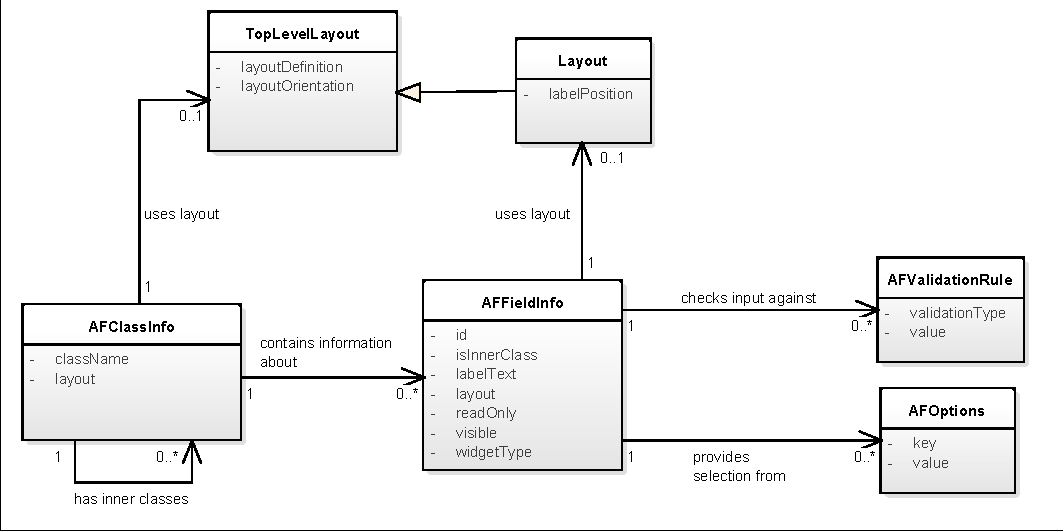
\includegraphics{images/domainModel}
\caption{Doménový model objektů obsahující metadata o objektu, nad kterým byla provedena inspekce}
\label{img:metadataModel}
\end{figure}

\subsubsection{AFMetaModelPack}
Tato třída zapouzdřuje informace, které popisují objekt, nad kterým byla prováděna inspekce. Třída rovněž slouží jako fasáda a nabízí programátorovi upravení metadat po generování. V případě serveru je toto návratový typ zdroje, na který klient přistoupí, chce-li znát metadata, která zdroj poskytuje.
\subsubsection{AFClassInfo}
Tato třída udržuje informace o hlavním objektu, z kterého je vytvářena definice. Třída má dále reference na své vnitřní proměnné a své potomky. Na základě generování dat je potřeba udržet pořadí, v kterém byla nad jednotlivými komponenty prováděna inspekce. V případě inspekce dat je i reference na neprimitivní datový typ jeho proměnná. Nicméně je potřeba, aby byl klient schopný určit, že se jedná o složitý datový typ a určit jeho pořadí v aktuálním objektu, aby mohl rozhodnout na jaké pozici objekt zobrazit. Z tohoto důvodu je ve třídě AFFieldInfo proměnná classType, která určuje, zdali se jedná o vnitřní třídu či primitivní datový typ.
\subsubsection{AFFieldInfo}
Tato třída je zodpovědná za poskytování detailních informací o proměnné objektu, nad kterým byla provedena inspekce. Třída udržuje název proměnné, widget, na který bude proměnná převedena, pravidla, která musí být splněna, název, pod kterým bude prezentována uživateli a zdali se jedná o složitý či jednoduchý objekt. Kromě těchto vlastností nese objekt také informace o tom, je-li komponenta viditelná a pouze pro čtení.
\subsubsection{AFRule}
Každá proměnná má souhrn vlastností, které musí být splněny. Typ widgetu ještě vždy nemusí určovat datový typ komponenty a neurčuje, je-li pole povinné či nikoliv. Tento soubor vlastností je popisován v této třídě. Třída využívá ENUM, který specifikuje podporované validace. Důvodem je to, že klient musí být schopný vytvořit tyto validační pravidla a interpretovat je na komponentě svým vlastním způsobem, který je specifický pro technologii, kterou používá. Jednou z dalších výhod je validace XML souboru, z kterého jsou pravidla vytvářena. Framework vytvoří pouze ty validační pravidla, která podporuje. Klient poté musí podporovaná pravidla interpretovat. 
\subsubsection{AFOptions}
Některé widgety umožňují, aby si uživatel vybral z několika předem připravených možností. Tyto možnosti musí být klientovi prezentovány. Tato třída udržuje informace o možnostech výběru v dané komponentě. Proměnná klíč je hodnota, která bude odeslána zpět na server a proměnná value je hodnota, která bude zobrazena klientovi. Tímto způsobem lze klientovi zobrazit jakýkoliv text, který bude zpětně mapován na jeho skutečnou hodnotu. Kromě textu lze samozřejmě zobrazit čísla či hodnoty výčtových typů.

\subsection{Server}
Server je zařízení či software, který umožňuje zpracovat požadavky od klientů a na jejich základě vytvořit odpověď. Server tedy poskytuje svým klientům určitý typ obsahu. Způsob a původ obsahu, který server poskytuje, je pro klienta povětšinou neznámý. V současné době je velmi populární přístup, při kterém server získá data z více zdrojů a poskytne je klientovi. Hovoříme o tzv. mashup \cite{Tuchinda2008}. Mashup nemusí být pouze z veřejných zdrojů, lze využít i privátní zdroje, či lze k sestavení odpovědi využít další služby. Klient napojený na server tohoto typu nemusí mít o těchto dalších zdrojích vůbec žádnou povědomost a dotazuje se pouze vůči tomuto serveru, který zpracovává jeho požadavky. 
Klientů, kteří získávají data z veřejných, či privátních zdrojů serveru může být celá řada. Mohou to být vlastní privátní aplikace, mobilní aplikace, Javascriptoví klienti či další server, který pouze využívá veřejné zdroje serveru k sestavení odpovědi svým vlastním klientům. V těchto případech je potřeba zvážit způsob generování definic dat, které by mohly způsobit stávajícím klientům problémy. V ideálním případě musí být framework integrován takovým způsobem, aby byla zachována stávající funkcionalita a framework ji pouze rozšířil. 
Ke generování definic objektů jsou potřeba následující věci:
\begin{enumerate}
\item Objekt, jehož definice budou generovány.
\item Mapování, na jehož základě bude rozhodnuto, o jaký typ komponenty půjde.
\item Definice komponenty včetně vlastností jako jsou validace, layout a popis chování komponenty.
\item Layout, ve kterém budou komponenty sestaveny.
\item Framework, který provede inspekci.
\item Framework, který bude inspekci řídit a bude interpretovat vygenerovaná data. Tento framework musí zároveň ověřit validitu jednotlivých komponent.
\end{enumerate}

Výše uvedené vlastnosti, nebudou mít vliv na změnu funkcionality. K inspekci a mapování bude využit framework AspectFaces \cite{aspectFaces}, který umožňuje na základě datových typů rozhodnout jakou komponentu využít. Definice komponent a jejich vlastností bude již v plné kompetenci vývojáře, nicméně základní komponenty a jejich chování bude předpřipraveno ve vzorovém projektu, aby se vývojář mohl inspirovat.

\subsection{Klient}
Klientská část frameworku bude vytvářet komponenty na základě metadat, která obdržela od serveru. Klient nebude mít žádnou znalost o objektech, které mu server poskytuje, předtím než obdrží jejich definice. Klient nicméně musí vědět, který zdroj mu poskytne relevantní definice a který ze zdrojů mu poskytne data odpovídající těmto definicím. Zároveň také musí vědět, na který zdroj data zpětně odeslat. Zdroj je obvykle specifikován následujícími parametry:
\begin{enumerate}
\item Adresa serveru
\item Port
\item Protokol
\item Metoda (get, post, put, delete)
\item Dodatečné hlavičkové parametry například content-type
\end{enumerate}
Klient tedy bude muset vždy specifikovat tyto parametry. Z hlediska použitelnosti je vhodné mít tyto specifikace v XML souboru, který bude umět klient jednoduše načíst. Pro usnadnění bude načítání provádět framework. Ukázka je na obrázku \ref{code:xmlSource}. V ukázkovém příkladu je specifikován zdroj s metadaty, který je vždy povinný. Zdroj se nachází na adrese\\ http://localhost:8080/AFServer/rest/users/loginForm. Zdroj s daty není specifikován, což způsobí, že ve formuláři nebudou žádná data. Formulář bude možné odeslat na adresu http://localhost:8080/AFServer/rest/users/login. Zdroj má identifikátor loginForm. V jednom XML dokumentu lze mít více zdrojů. K vložení dat do konkrétního zdroje lze využít EL. V hlavičce může být 0 až N parametrů, přičemž každý parametr musí být uveden ve stejném formátu, jako je znázorněno na obrázku \ref{code:xmlSource}. Obdobný způsob se využívá v JavaEE aplikací v deskriptoru web.xml. Klient umí sestavit požadavek na základě tohoto popisu a interpretovat odpověď od serveru. Není tedy nutné, aby uživatel implementoval třídy, které se umožní aplikaci připojení na server a získání dat.

\begin{lstlisting}[caption=Ukázka XML specifikace zdrojů,
label={code:xmlSource}, basicstyle=\footnotesize]
<?xml version="1.0" encoding="UTF-8"?>
<connectionRoot xmlns:xsi="http://www.w3.org/2001/XMLSchema-instance">
	<connection id="loginForm">
		<metaModel>
			<endPoint>localhost</endPoint>
			<endPointParameters>/AFServer/rest/users/loginForm</endPointParameters>
			<protocol>http</protocol>
			<port>8080</port>
			<header-param>
				<param>content-type</param>
				<value>Application/Json</value>
			</header-param>
		</metaModel>
		<send>
			<endPoint>localhost</endPoint>
			<endPointParameters>/AFServer/rest/users/login</endPointParameters>
			<protocol>http</protocol>
			<port>8080</port>
			<method>post</method>
			<header-param>
				<param>content-type</param>
				<value>Application/Json</value>
			</header-param>
		</send>
	</connection>
</connectionRoot>
\end{lstlisting}

Je patrné, že klient je schopný získat definice formulářů či tabulek, naplnit je daty a poté odeslat zpět na server. Důvodem, proč je klient schopný generovat formuláře na základě definice ze serveru je ten, že klient pracuje se stejnými objekty, které popisují metadata, jako server. Prozatím je k dispozici pouze strohý popis dat. Klientská část musí nyní rozhodnout jak data interpretovat, jak s nimi pracovat, jakým způsobem je validovat, jak je znovu sestavit a odeslat na server. Důležitým prvkem je i způsob uspořádání jednotlivých prvků, jejich velikosti, barvy a texty.

Využití frameworku by obdobně jako v případě serveru nemělo mít vliv na stávající použití aplikace. V případě referenčního řešení ve Swingu generuje klient JPanel, který lze vkládat do dalších panelů a vývojář tak není nikterak omezen, co se týče stávající aplikace. 

\begin{figure}[h!]
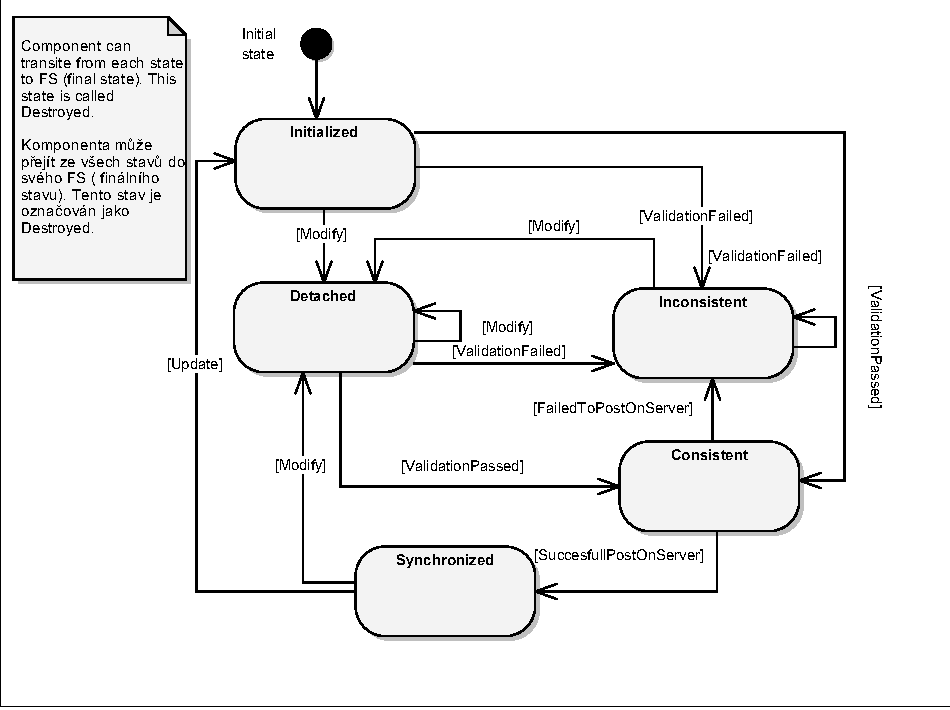
\includegraphics{images/formLifecCycle}
\caption{Životní cyklus formuláře}
\label{img:formLifeCycle}
\end{figure}

\subsection{Životní cyklus formuláře}
Formulář, jako každá komponenta, má svůj životní cyklus. Jeho stavy jsou znázorněny na obrázku \ref{img:formLifeCycle}. Formulář je po vygenerování a po naplnění daty v inicializačním stavu. V tomto stavu může být komponenta nevalidní, neboť data, která obdržela, nemusí splňovat požadované validace. K této situaci může dojít, je-li například přidána nová proměnná do datového modelu. Toto přidání obvykle probíhá tak, že se v koncové databázi, pokud jí software má, přidá políčko a nastaví se mu defaultní hodnota pro již existující data, která může být například null. V definici může být pole označeno jako povinné, avšak ve formuláři nemusí být vyplněno, což způsobí, že jsou data nevalidní, byť uživatel ve formuláři data nezměnil. Komponenta se pak přepne do stavu Inconsistent. V případě modifikace dat se komponenta dostává do stavu Detached. Tento stav značí, že byla data změněná. Pokud uživatel data stále mění, pak komponenta zůstává v tomto stavu. Ze stavu Detached přechází komponenta v případě úspěšné validace do stavu Consistent. V případě neúspěšné validace se komponenta dostane do stavu Inconsistent. Z tohoto stavu lze přejít pouze do dvou stavů jedním z nich je stav Detached. Do tohoto stavu lze přejít, pokud uživatel změní data ve formuláři. Komponenta může také zůstat ve stavu Inconsistent, pokud uživatel data nezmění a zkusí provést validaci znovu a tato validace opět selže. Konzistentní stav značí, že je komponenta připravená k odeslání dat na server. Pokud odeslání dat selže je komponenta přepnuta do stavu Inconsistent. V případě úspěšného odeslání dat, je komponenta přepnuta do stavu Synchronized. Ze stavu Synchronized lze přejít do stavu Initialized, pokud jsou data znovu načtena ze serveru a do stavu Detached, pokud jsou data upravena uživatelem.

\section{Případy užití}
Případy užití a jejich scénáře \cite{UmlArlow} specifikují chování systému. V této práci lze nahlížet na případy užití ze dvou stran. První z nich je koncový uživatel, neboli vývojář, který framework využívá. Druhým z nich je samotný framework, který provádí akce, aby splnil úkol, který mu uživatel uložil. V této sekci se zaměříme na případy užití koncového uživatele, které specifikují použití frameworku. Na obrázku \ref{img:useCase} jsou zachyceny všechny tyto případy užití. Pro ukázku detailně rozebereme případ užítí na obrázku \ref{img:useCaseSmall}. Na tomto případu je znázorněno odeslání dat z vygenerovaného formuláře zpět na server. Součástí je samozřejmě validace zadaných dat a jejich zpětné sestavení, neboť formulář byl vytvořen na základě metadat a klient tedy zná pouze strukturu objektu popsanou těmito metadaty. 
\begin{figure}[h!]
\begin{center}
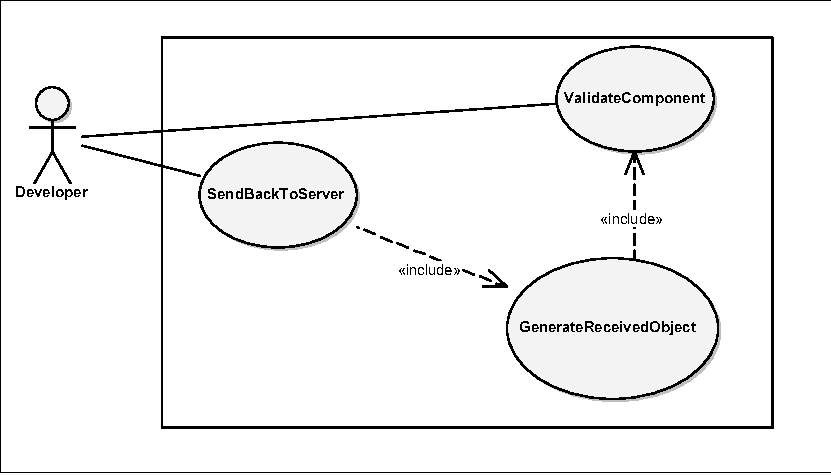
\includegraphics{images/useCaseSmall}
\caption{Část případů užití znázorňující odeslání dat na server z vygenerovaného formuláře}
\label{img:useCaseSmall}
\end{center}
\end{figure}
\subsubsection{Validace komponenty}
Tento případ užití je znázorněn na obrázku \ref{img:useCaseSmall} a jmenuje se ValidateComponent.

Případ užití: Validace komponenty\\
ID: 1\\
Popis: 
Uživatel využívá framework ke generování formulářů. Hlavním úkolem formuláře je možnost vkládat či upravovat data a odesílat je zpět na server. Před odesláním dat na server musí být provedena validace, aby se zajistilo, že bude formát dat serveru vyhovovat a bude umět s daty pracovat.
\\
Aktér: Uživatel\\
Vstupní podmínky:
\begin{enumerate}
\item Formulář musí být sestaven na základě metadat a framework musí znát formulář, s kterým chce pracovat.
\end{enumerate}
Scénář:
\begin{enumerate}
\item Případ užití začíná obdržením požadavku od uživatele žádající validaci dat.
\item Systém vyhledá pole k validaci.
\item Dokud existují pole k validaci pak:
\begin{enumerate}
\item Systém získá konkrétní pole k validaci.
\item Systém určí typ komponenty a požádá builder, který ji sestavil o data.
\item Dokud existuje validace, která zatím nebyla na poli vykonána pak:
\begin{enumerate}
\item Systém požádá validátor o validaci.
\item Pokud validace selže pak:
\begin{enumerate}
\item Systém ukončí validování tohoto pole a zobrazí u něj chybové validační hlášení.
\end{enumerate}
\end{enumerate}
\end{enumerate}
\end{enumerate}

Případ užití: Sestavení dat\\
ID: 2\\
Popis: 
Uživatel využívá framework ke generování formulářů. Hlavním úkolem formuláře je možnost vkládat či upravovat data a odesílat je zpět na server. Před odesláním dat na server musí být tyto data zpětně sestaveny, aby s nimi server dokázal pracovat.
\\
Aktér: Uživatel\\
Vstupní podmínky:
\begin{enumerate}
\item Formulář musí být sestaven na základě metadat a framework musí znát formulář, se kterým chce pracovat. Framework musí znát formát dat, která server očekává.
\end{enumerate}
Scénář:
\begin{enumerate}
\item Případ užití začíná obdržením požadavku od uživatele žádající sestavení dat z formuláře.
\item Zahrnout(Validace komponenty).
\item Pokud validace dopadla úspěšně pak:
\begin{enumerate}
\item Systém získá pole, která budou odeslána.
\item Pokud existuje pole, které ještě nebylo transformováno pak:
\begin{enumerate}
\item Systém určí typ komponenty a požádá builder, který ji sestavil, o data.
\item Systém určí název proměnné a třídu, do které patří, a nastaví jí data.
\end {enumerate}
\item Systém na základě formátu dat, které server očekává, rozhodne, v jakém formátu data zaslat a převede je na daný formát.
\end{enumerate}
\end{enumerate}

Výstupní podmínka:
\begin{enumerate}
\item Data ve formuláři byla převedena na objekt, s kterým umí server pracovat.
\end{enumerate}

Případ užití: Odeslání dat\\
ID: 3\\
Popis: 
Uživatel využívá framework ke generování formulářů. Hlavním úkolem formuláře je možnost vkládat či upravovat data a odesílat je zpět na server. Před odesláním dat na server musí být tato data zpětně sestavena, aby s nimi server dokázal pracovat, a musí splnit validační kritéria.
\\
Aktér: Uživatel\\
Vstupní podmínky:
\begin{enumerate}
\item Formulář musí být sestaven na základě metadat a framework musí znát formulář, se kterým chce pracovat. Framework musí znát zdroj, na který mají být data odeslána, a všechny potřebné informace, které zdroj vyžaduje.
\end{enumerate}
Scénář:
\begin{enumerate}
\item Případ užití začíná obdržením požadavku od uživatele žádající odeslání formuláře na server.
\item Zahrnout(Validace komponenty).
\item Zahrnout(Sestavení dat)
\item Dokud je validace či sestavení dat neúspěšné pak:
\begin{enumerate}
\item Systém zobrazí chybové hlášení a určí, u kterých polí nastala chyba.
\item Uživatel chybu opraví a požádá systém o opětovnou validaci a sestavení dat.
\end{enumerate}
\item Systém vytvoří připojení na specifikovaný zdroj a odešle data.
\item Pokud odeslání selhalo pak:
\begin{enumerate}
\item Systém zobrazí chybové hlášení, že nebylo možné data odeslat včetně odpovědi od serveru, je-li nějaká.
\end{enumerate}
\end{enumerate}

Výstupní podmínka:
\begin{enumerate}
\item Data byla odeslána.
\end{enumerate}


\section{Omezení frameworku}
Existují určité možnosti, které nebudou ve frameworku podporovány. V následujícím přehledu budou představeny nepodporované vlastnosti frameworku v aktuální verzi.
\begin{enumerate}
\item Inspekce datových proměnných typu List a Array
\item Získávání dat ve formátu XML. Framework plně podporuje JSON.
\item Customizace jednotlivých polí. Framework podporuje customizaci formuláře a všech jeho polí, nicméně nedisponuje možností přizpůsobovat jednotlivá pole.
\item Framework neumožňuje v jednom poli reprezentovat složený datový typ. Například třídu.
\item Odesílání dat a validace dat v tabulce. Tabulka je v této verzi pouze readonly.
\item Framework vyžaduje ke své funkčnosti jak serverovou tak klientskou stranu. V případě, že klientské straně chybí serverová strana, tak je framework nefunkční. V případě, že serverové straně chybí klientská strana, tak je serverová strana stále schopná vytvářet definice dat.
\item Klientská strana zobrazuje pouze ta data, která obdržela od serveru, nelze vytvářet automatický Mashup na klientovi. Nicméně klient může generovaný formulář umístit mezi jiné komponenty.
\item Klientská strana nedokáže sestavit objekt, který získala z metadat do takové míry aby z něj byla schopná vytvořit instanci. Neboli klientská strana si neudržuje konkrétní objekt, který obdržela, pouze jeho popis.
\item Serverová část využívá k automatické inspekci framework. Bez tohoto frameworku není možné inspekci provést, nicméně uživatel si může definovat svou vlastní definici bez nutnosti inspekce dat.
\end{enumerate}

\section{Uživatelé a zabezpečení}
Téměř každá aplikace využívá způsob, při kterém se uživatel autentizuje a aplikace mu na základě jeho rolí přidělí oprávnění. V případě využití bez stavového protokolu, jakým REST je lze posílat informace o uživateli v hlavičce požadavku. Tyto informace mohou být samozřejmě zašifrované. Framework podporuje vkládání libovolných informací do hlavičky requestu. Klient si také může zvolit, zdali bude využívat http či https protokol. Velmi rozšířenou možností je využitý Oauth. Jednou z možností, je vložení parametrů do hlavičky či do adresy. Vkládání dynamických adres či proměnných do hlavičky requestu framework podporuje. 

Druhou části jsou uživatelské role, na základě kterých se generuje uživatelské rozhraní. Serverová část využívá framework AspectFaces \cite{aspectFaces}, který podporuje uživatelské role v systému. Je jen na programátorovi, jaký framework na autentizaci a autorizaci na straně serveru použije. Jednou z možností je například napsat si vlastni interceptor, který určí, o jakého uživatele se jedná, přiřadí mu roli v systému, na základě které se mu zobrazí konkrétní obsah. Server při generování metadat může využít různé mapovací soubory na základě uživatelské role. Specifikace tohoto chování je opět v plné kompetenci uživatele.
\section{Použité technologie}
V následující sekci jsou rozebrány použité technologie. Kromě samotného frameworku je součástí práce i ukázkový projekt na platformě JavaEE a JavaSE.
\subsection{Java SE - Swing}
Klientská část frameworku je schopná vygenerovat formuláře či tabulky a naplnit je daty a data odeslat. Klientská část je přizpůsobena frameworku Swing. Důvodem je, že vývoj Swingové aplikace je rychlý a Swing zná velké množství vývojářů, kteří si framework mohou jednoduše otestovat. Nicméně metadata, která server generuje lze interpretovat v jakékoliv technologii. Swing je knihovna grafických a uživatelských prvků. Poskytuje komponenty, layouty, actionListenery, okna, dialogová okna a další prvky, pomocí kterých lze vytvářet interaktivní aplikace.
\subsection{Java EE}
Java EE je platforma sloužící k vývoji enterprise aplikací. V současné době je oblíbená jak u velkých tak u menších korporací. Java EE přináší podporu pro Restové služby, JFS, JSP, EJB, databázové frameworky, anotace a další komponenty. Aplikace v JavaEE se obvykle nasazuje na aplikační server. Aplikační servery mohou být v cloudu a podílet se společně na zpracování requestů. Důvodem využití této platformy je fakt, že klient vytváří requesty vůči serveru a server tato data zpracovává. Je vhodné mít na serveru platformu, která je ověřená a má potenciál ke zpracování těchto requestů. V této práci generujeme data pomocí restového rozhraní a Java EE splňuje specifikaci, které se tohoto rozhraní týká. 
\subsection{AspectFaces}
AspectFaces je framework, který umí provádět inspekci nad zadanými objekty a na základě datových typů a dalších parametrů rozhodovat o to, jaká komponenta se použije pro konkrétní datový typ. Framework využívá AspectFaces k tomu, aby provedl toto mapování a sestavil popis uživatelského rozhraní. Hlavním důvodem využití tohoto frameworku je fakt, že je distribuován jako open source pod licencí LGPL v3 a že lze využít jeho funkcionalitu ke statické inspekci dat. Tato inspekce je již odladěna a není tedy důvod psát znovu již vynalezenou věc. 
\subsection{Ukázkový projekt}
Ukázkový projekt demonstruje použití frameworku. Skládá se ze dvou částí. Klientské a serverové. Klientská část využívá pouze Swing. Serverová část je mnohem sofistikovanější a využívá aktuální technologie. Ukázkový projekt zde znázorňuje použítí frameworku a jeho omezení. Ukázkový projekt je koncipován, tak aby ho bylo možné nasadit bez nutnosti dodatečného nastavení.
\subsubsection{GlassFish}
GlassFish \cite{glassfish} je open source aplikační server, jedná se o certifikovaný server JavaEE. Umožňuje clustering, monitoring, podporu EJB, REST a JDBC. Architektura jádra je založena na frameworku OSGI, který umožňuje vzdáleně přidávat, startovat či ukončovat komponenty bez nutnosti restartování celého serveru. Důvodem proč je Glassfish využit na tomto projektu je čistě demonstrativní. Nicméně, každý aplikační server má svá specifika, a proto je ukázková aplikace odladěna právě pro GlassFish. Jak již bylo zmíněno Glassfish distribuje vestavěnou podporou pro Rest a umožňuje použití Derby DB v režimu in-memory bez nutnosti speciálního nastavení.
\subsubsection{RestEasy}
Jedná se o framework, pomocí kterého lze vytvářet RESTful aplikace. Tento framework může běžet v libovolném servletovém kontajneru. Framework podporuje například JSON, XML serializace objektů, EJB a je splňuje JAX-RS implementaci. Tvorba aplikací s restovým rozhranním je tak díky tomuto frameworku mnohem jednodušší a vývoj je rychlejší. 
\subsubsection{EJB}
Enterprise JavaBeans \cite{javaEETutorial} jsou serverově orientované komponenty, které zapouzdřují business logiku a přístup do databáze. Jsou spravovány v rámci serverového kontejneru, který zajišťuje jejich vytvoření i odstranění z paměti. EJB mohou být různých typů.
\begin{itemize}
\item Stateless
\item Statefull
\item Singleton
\end{itemize}
Jak již bylo zmíněno, o jejich správu se stará serverový kontejner, nemusíme tedy řešit problémy spojené s vytvořením a destrukcí singletonu \cite{gamma}. Mezi hlavní výhody EJB patří transakční zpracování, zajištění systémových služeb a bezpečnostní autorizace. Abychom definovali či~získali přístup k těmto třídám, používáme anotace, které jsou velmi dobře čitelné a~srozumitelné.
\subsection{Derby DB}
V ukázkovém projektu je potřeba data ukládat do databáze. Při vytváření byl kladen důraz na to, aby noví uživatelé nemuseli v konfiguračních souborech specifikovat nastavení a mohli ukázkový projekt ihned nasadit a vyzkoušet. Z tohoto důvodu je využita light databáze Derby. Ukázkový projekt ji využívá v in-memory módu, což znamená, že budou data po zastavení serveru ztracena. Spolu s Derby DB využívá ukázkový projekt ORM s defaultním nastavením na create. Po startu aplikace jsou v čisté databázi vytvořeny požadované tabulky, které odráží definice objektů, jenž jsou anotované jako entity. Další výhodou je možnost využít anotací k nastavení validací přímo na databázi. Tyto validace pak mohou být využity při inspekci dat a na jejich základě mohou být vytvořeny validace, či konkrétní komponenty.

%*****************************************************************************
% Seznam literatury je v samostatnem souboru reference.bib. Ten
% upravte dle vlastnich potreb, potom zpracujte (a do textu
% zapracujte) pomoci prikazu bibtex a nasledne pdflatex (nebo
% latex). Druhy z nich alespon 2x, aby se poresily odkazy.

% originally following specification for bibliography formating was used
%\bibliographystyle{abbrv}

% Here is an improvment by Petr Dlouhy (April 2010).
% It is mainly for supervisors who expect Czech fomrating rules for references
% Additional feature is live url addresses to sources from your pdf file
% It requires the file csplainnat.bst (included in this sample zipfile).
\bibliographystyle{csplainnat}

%bibliographystyle{plain}
%\bibliographystyle{psc}
{
%JZ: 11.12.2008 Kdo chce mit v techto ukazkovych odkazech take odkaz na CSTeX:
\def\CS{$\cal C\kern-0.1667em\lower.5ex\hbox{$\cal S$}\kern-0.075em $}
\bibliography{reference}
}
%%%%%%%%%%%%%%%%%%%%%%%%%% 
% vše co následuje bude uvedeno v přílohách
\appendix	

\printnomenclature
\label{apx:zkratky}

\chapter{Obsah přiloženého CD}
\textbf{\large Tato příloha je povinná pro každou práci. Každá práce musí totiž obsahovat přiložené CD. Viz dále.}

Může vypadat například takto. Váš seznam samozřejmě bude odpovídat typu vaší práce. (viz \cite{infodp}):

\begin{figure}[h]
\begin{center}
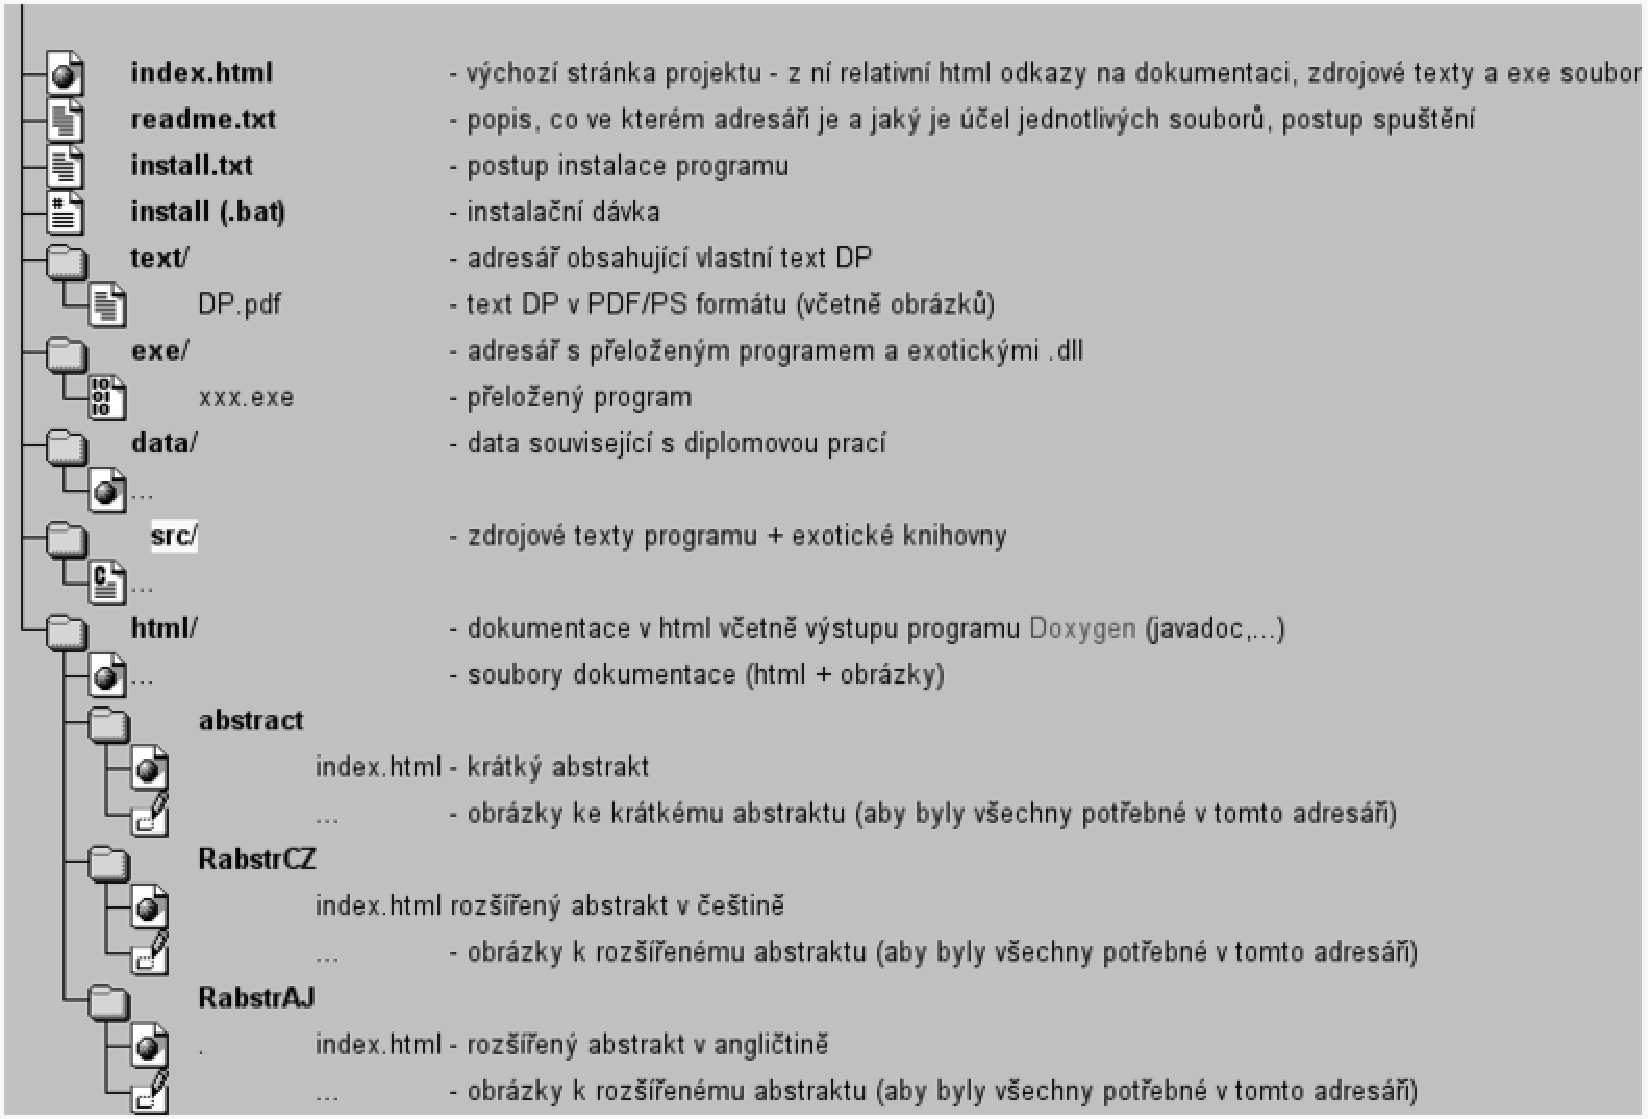
\includegraphics[width=14cm]{figures/seznamcd}
\caption{Seznam přiloženého CD --- příklad}
\label{fig:seznamcd}
\end{center}
\end{figure}

Na GNU/Linuxu si strukturu přiloženého CD můžete snadno vyrobit příkazem:\\ 
\verb|$ tree . >tree.txt|\\
Ve vzniklém souboru pak stačí pouze doplnit komentáře.

Z \textbf{README.TXT} (případne index.html apod.)  musí být rovněž zřejmé, jak programy instalovat, spouštět a jaké požadavky mají tyto programy na hardware.

Adresář \textbf{text}  musí obsahovat soubor s vlastním textem práce v PDF nebo PS formátu, který bude později použit pro prezentaci diplomové práce na WWW.

\end{document}
